\documentclass[10pt,a4paper]{article}

\usepackage{appendix}
\usepackage{graphicx}
\usepackage{biblatex}
\usepackage{parskip}
\usepackage{listings}
\usepackage{caption}
\usepackage{subcaption}
\usepackage{amsmath}
\usepackage{listings}
\usepackage{xcolor}
\usepackage[most]{tcolorbox}

%%%%%%%%%%%%%%%%%%%%%%%%%%%%%%%%%%%%%%%%%%%%%%%%%%%%%%%%%%%%%%%%%%%%%%%%%%%%%%%%%%%%%%%%%%%%%%%%%%%%%%%%%%
\definecolor{codegreen}{rgb}{0,0.6,0}
\definecolor{codegray}{rgb}{0.5,0.5,0.5}
\definecolor{codepurple}{rgb}{0.58,0,0.82}
\definecolor{backcolour}{rgb}{1,1,1}

\lstdefinestyle{mystyle}
{
  backgroundcolor=\color{backcolour},  
  commentstyle=\color{codegreen},
  keywordstyle=\color{magenta},
  numberstyle=\tiny\color{codegray},
  stringstyle=\color{codepurple},
  basicstyle=\ttfamily\footnotesize,
  breakatwhitespace=false,     
  breaklines=true,         
  captionpos=b,          
  keepspaces=true,         
  numbers=left,          
  numbersep=5pt,         
  showspaces=false,        
  showstringspaces=false,
  showtabs=false,         
  tabsize=2
}

\lstset{style=mystyle}
%%%%%%%%%%%%%%%%%%%%%%%%%%%%%%%%%%%%%%%%%%%%%%%%%%%%%%%%%%%%%%%%%%%%%%%%%%%%%%%%%%%%%%%%%%%%%%%%%%%%%%%%%%

\lstset{basicstyle=\ttfamily, breaklines = true, tabsize=2}
\graphicspath{ {./Images/} }
\setlength{\parskip}{1em}
\begin{document}
%%%%%%%%%%%%%%%%%%%%%%%%%%%%%%%%%%%%%%%%%%%%%%%%%%%%%%%%%%%%%%%%%%%%%%%%%%%%%%%%%%%%%%%%%%%%%%%%%%%%%%%%%%

\begin{titlepage}
	\centering
	{\scshape\LARGE Imperial College London \par}
	\vspace{1cm}
    {\scshape\Large Computer Architecture: Year 2\par}
    \vspace{1.5cm}
	{\huge\bfseries 0: Computer abstraction \par}
	\vspace{2cm}
	{\Large\ Xin Wang }
	\vfill
	{\large \today\par}
\end{titlepage}

%%%%%%%%%%%%%%%%%%%%%%%%%%%%%%%%%%%%%%%%%%%%%%%%%%%%%%%%%%%%%%%%%%%%%%%%%%%%%%%%%%%%%%%%%%%%%%%%%%%%%%%%%%

\tableofcontents
\pagebreak

%%%%%%%%%%%%%%%%%%%%%%%%%%%%%%%%%%%%%%%%%%%%%%%%%%%%%%%%%%%%%%%%%%%%%%%%%%%%%%%%%%%%%%%%%%%%%%%%%%%%%%%%%%
\section{Introduction}

Programmers are always concerned about the performance of programs because getting results to the
user quickly is critical. In the past where primary constraint on computer performance was the size
of the computer’s memory, minimising the memory space was the way to make programs fast. In the
present, advances in computer design and memory technology have reduced the importance of memory.

Programmers now need to understand the issues such as the parallel nature of processors, the
hierarchical nature of memories and the energy efficiency of their programs running locally or in
the Cloud.

The questions that are of concern to be covered are:
\begin{itemize}
    \item Understanding the gap between hardware and software i.e. how programs written in a
    high-level language such as C or Java are translated into the hardware language and how
    does the hardware execute the resulting program.
    \item Bridging the gap between hardware and software i.e. the interface between the software and
    the hardware, how software instruct the hardware to perform needed functions.
    \item Factors determining the performance of a program and techniques used to improve it.
    \item The reasons for and the consequences of the recent switch from sequential processing to parallel processing.
\end{itemize}

%%%%%%%%%%%%%%%%%%%%%%%%%%%%%%%%%%%%%%%%%%%%%%%%%%%%%%%%%%%%%%%%%%%%%%%%%%%%%%%%%%%%%%%%%%%%%%%%%%%%%%%%%%
\subsection{Eight great ideas of computer architecture}

\begin{enumerate}
    \item \textbf{Design for Moore's Law}: The one constant for computer designers is rapid change, driven largely by Moore’s Law stating that integrated circuit resources double every 18–24 months.
    \item \textbf{Abstraction to simplify design}: A productivity technique for hardware and
    software by using abstractions to represent the design at different levels of representation
    e.g. lower-level details are hidden to offer a simpler model at higher levels.
    \item \textbf{Making the common case fast}: Making the common case fast will tend to enhance
    performance better than optimising the rare case. 
    \item \textbf{Performance via parallelism}: Designs that get more performance by performing operations in parallel.
    \item \textbf{Performance via pipelining}: A particular pattern of parallelism prevalent in
    computer architecture. 
    \item \textbf{Performance via prediction}: Sometimes it is faster on average to guess an action
    and start processing assuming that the mechanism to recover from a mis-prediction is not too
    expensive and the prediction is relatively accurate.
    \item \textbf{Hierarchy of memories}: The goal is for memory to be fast, large, and cheap since
    as memory speed shapes performance, capacity limits size of problems, and cost of memory
    determines the cost of computers for the consumer. Commonly addressed with a hierarchy of memories, with 
    the fastest, smallest, and most expensive memory per bit and the slowest, largest, and cheapest
    per bit.
    \item \textbf{Dependability via redundancy}: Computers need to be fast and dependable. Systems
    are made dependable by including redundant components that can take over when a failure occurs and to help detect failures.
\end{enumerate}

%%%%%%%%%%%%%%%%%%%%%%%%%%%%%%%%%%%%%%%%%%%%%%%%%%%%%%%%%%%%%%%%%%%%%%%%%%%%%%%%%%%%%%%%%%%%%%%%%%%%%%%%%%
\section{Computer structure organisation}

The computer structure can be abstracted into three levels: Applications, Operating system and
Hardware. \par
\begin{figure} [h!]
    \centering
    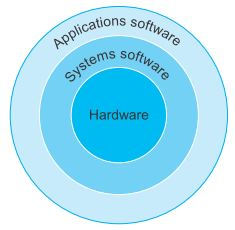
\includegraphics[scale=0.7]{Three layer.JPG}
\end{figure}
The modern multilevel view spilts it into six layers:
\begin{figure} [h!]
    \centering
    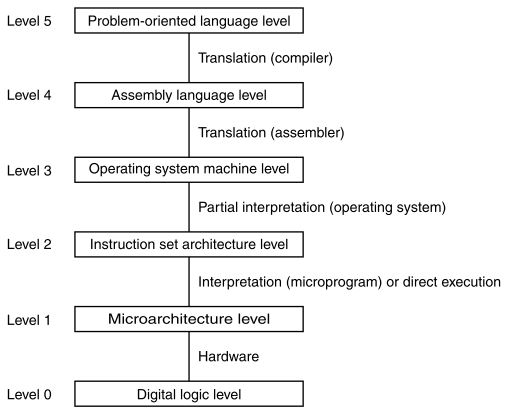
\includegraphics[scale=0.8]{Six layer.JPG}
\end{figure}
\begin{itemize}
    \item \textbf{Level 5}: Consists of languages designed to be used by applications programmers to
    solve problem e.g. Python and C++. Programs written are generally translated to level 4 by
    \textbf{compilers}, although occasionally they are interpreted instead.
    \begin{tcolorbox}[breakable,colback=white]
    \textbf{Compiler}: A program that translates high-level language statements into assembly
    language statements.
    \end{tcolorbox}
    \item \textbf{Level 4}: Intended primarily for running the interpreters and assemblers needed to support the higher levels.
    \begin{tcolorbox}[breakable,colback=white]
    \textbf{Assembler}:  A program that translates a symbolic version of instructions into the binary version.
    \end{tcolorbox}
    \item \textbf{Level 3}: The operating system level.
    \item \textbf{Level 2}: The Instruction Set Architecture level. Every
    computer manufacturer publishes a manual describing the instructions carried out interpretively
    by the microprogram or hardware execution circuits. 
    \item \textbf{Level 1}: At this level a collection of $8$ to $32$ registers form local memory
    and the ALU which is capable of performing simple arithmetic operations. The registers are
    connected to the ALU to form a data path.
    \item \textbf{Level 0}: Logic gates built from transistors to form a register.
\end{itemize}


%%%%%%%%%%%%%%%%%%%%%%%%%%%%%%%%%%%%%%%%%%%%%%%%%%%%%%%%%%%%%%%%%%%%%%%%%%%%%%%%%%%%%%%%%%%%%%%%%%%%%%%%%%
\end{document}